\section{Compiladores}
Un compilador no es mas que un programa que basicamente, toma el codigo C 
y lo traduce a codigo de maquina. Existen varios para C, como ser GCC, Clang y el Compilador de Intel. 
Lo que hicimos fue compilar los filtros con GCC y clang, teniendo como hipotesis que GCC anda mejor, pues en caso contrario clang vendria instalado por defecto en vez de GCC.
Las versiones que vamos a utilizar para comparar son 5.3.1 para GCC y 3.8.0 para Clang
%Lo que vamos a hacer es compilar el codigo con Clang/GCC y ver si encontramos diferencias.Para comparar, se van a usar la version 4.8.4 de GCC y la 3.4 de Clang. 
%Para realizar la comparacion, vamos a compilar el TP con GCC y luego con Clang.
%Para empezar, vamos a comparar con optimizacion nula
Aqui el grafico de GCC

\begin{figure}[H]
    \centering
    \begin{floatrow}
      \ffigbox[\FBwidth]{\caption{Filtros con GCC -O0}}{%
        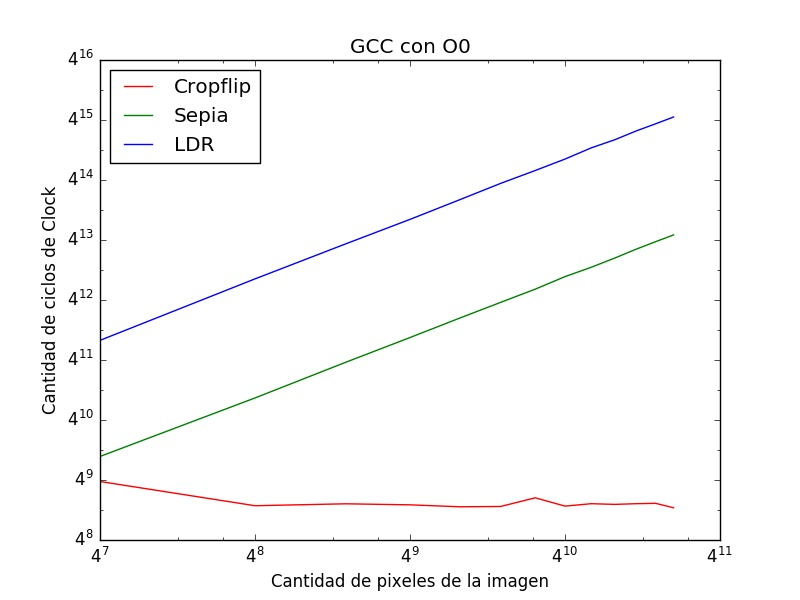
\includegraphics[scale=.50]{./imagenes/GCC0.jpg}   
      }
    \end{floatrow}
\end{figure}


Aca vemos que Cropflip, es el filtro mas rapido. Es esperable ya que solo hace accesos a memoria mientras que sepia y cropflip hace operaciones arimeticas

Aqui el grafico de Clang

\begin{figure}[H]
    \centering
    \begin{floatrow}
      \ffigbox[\FBwidth]{\caption{Filtros con Clang -O0}}{%
        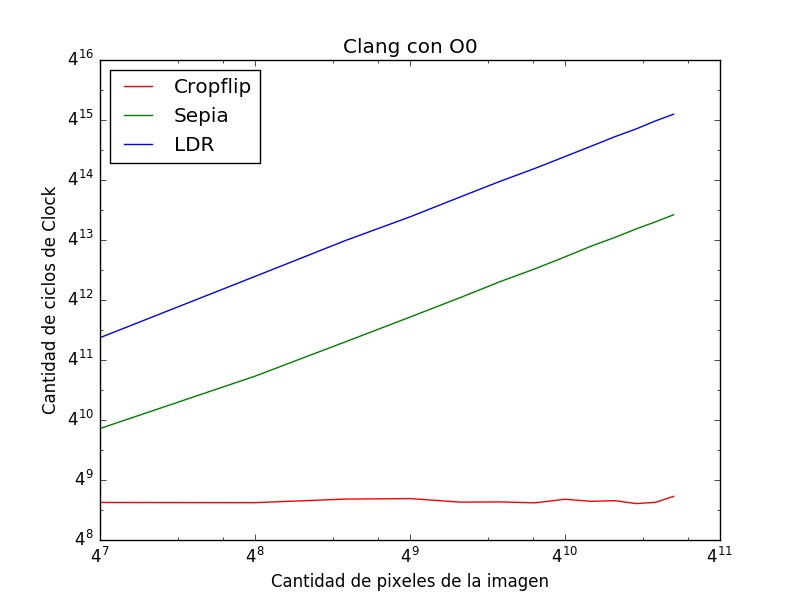
\includegraphics[scale=.50]{./imagenes/Clang0.jpg}   
      }
    \end{floatrow}
\end{figure}

Vemos que en Cropflip gana Clang, pero en Sepia y LDR gana GCC, en sepia es mas notorio mientras que en LDR la diferencia es bastante menor.


Ahora, vamos a repetir el mismo experimento pero variando las flags, esta vez vamos a usar 03 y como hipotesis, esperamos ver un comportamiento similar al visto en O0.
\begin{figure}[H]
    \centering
    \begin{floatrow}
      \ffigbox[\FBwidth]{\caption{Filtros con GCC -O0}}{%
        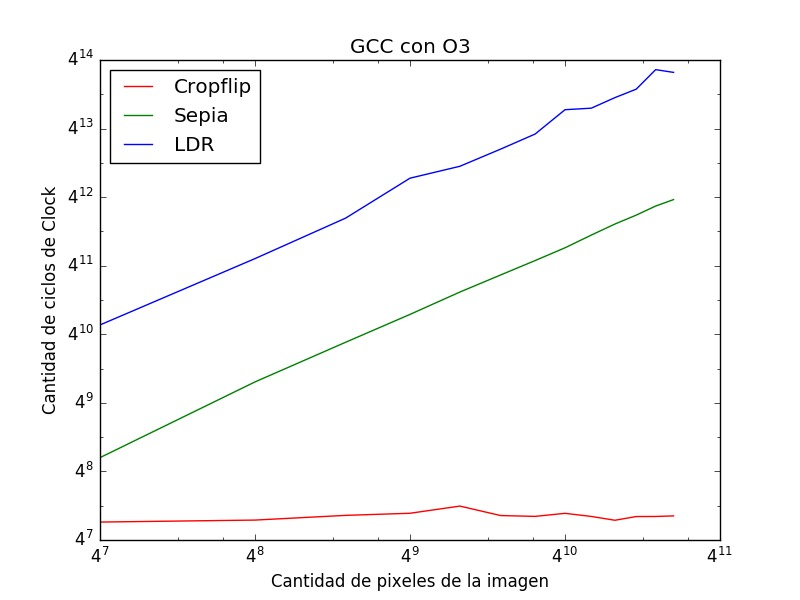
\includegraphics[scale=.50]{./imagenes/GCC3.jpg}   
      }
    \end{floatrow}
\end{figure}


\begin{figure}[H]
    \centering
    \begin{floatrow}
      \ffigbox[\FBwidth]{\caption{Filtros con Clang -O0}}{%
        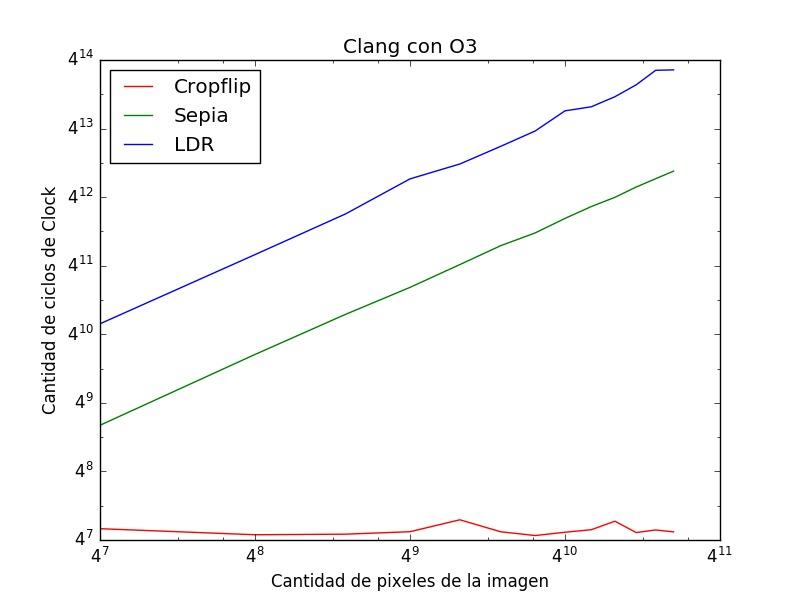
\includegraphics[scale=.50]{./imagenes/Clang3.jpg}   
      }
    \end{floatrow}
\end{figure}

Efectivamente, se da el comportamiento previsto, en Cropflip gana Clang mientras que en los otros gana GCC


